\documentclass{ximera}

%\usepackage{todonotes}

\newcommand{\todo}{}

\usepackage{esint} % for \oiint
\ifxake%%https://math.meta.stackexchange.com/questions/9973/how-do-you-render-a-closed-surface-double-integral
\renewcommand{\oiint}{{\large\bigcirc}\kern-1.56em\iint}
\fi


\graphicspath{
  {./}
  {ximeraTutorial/}
  {basicPhilosophy/}
  {functionsOfSeveralVariables/}
  {normalVectors/}
  {lagrangeMultipliers/}
  {vectorFields/}
  {greensTheorem/}
  {shapeOfThingsToCome/}
  {dotProducts/}
  {partialDerivativesAndTheGradientVector/}
  {../productAndQuotientRules/exercises/}
  {../normalVectors/exercisesParametricPlots/}
  {../continuityOfFunctionsOfSeveralVariables/exercises/}
  {../partialDerivativesAndTheGradientVector/exercises/}
  {../directionalDerivativeAndChainRule/exercises/}
  {../commonCoordinates/exercisesCylindricalCoordinates/}
  {../commonCoordinates/exercisesSphericalCoordinates/}
  {../greensTheorem/exercisesCurlAndLineIntegrals/}
  {../greensTheorem/exercisesDivergenceAndLineIntegrals/}
  {../shapeOfThingsToCome/exercisesDivergenceTheorem/}
  {../greensTheorem/}
  {../shapeOfThingsToCome/}
  {../separableDifferentialEquations/exercises/}
  {vectorFields/}
}

\newcommand{\mooculus}{\textsf{\textbf{MOOC}\textnormal{\textsf{ULUS}}}}

\usepackage{tkz-euclide}
\usepackage{tikz}
\usepackage{tikz-cd}
\usetikzlibrary{arrows}
\tikzset{>=stealth,commutative diagrams/.cd,
  arrow style=tikz,diagrams={>=stealth}} %% cool arrow head
\tikzset{shorten <>/.style={ shorten >=#1, shorten <=#1 } } %% allows shorter vectors

\usetikzlibrary{backgrounds} %% for boxes around graphs
\usetikzlibrary{shapes,positioning}  %% Clouds and stars
\usetikzlibrary{matrix} %% for matrix
\usepgfplotslibrary{polar} %% for polar plots
\usepgfplotslibrary{fillbetween} %% to shade area between curves in TikZ
%\usetkzobj{all}
\usepackage[makeroom]{cancel} %% for strike outs
%\usepackage{mathtools} %% for pretty underbrace % Breaks Ximera
%\usepackage{multicol}
\usepackage{pgffor} %% required for integral for loops



%% http://tex.stackexchange.com/questions/66490/drawing-a-tikz-arc-specifying-the-center
%% Draws beach ball
\tikzset{pics/carc/.style args={#1:#2:#3}{code={\draw[pic actions] (#1:#3) arc(#1:#2:#3);}}}



\usepackage{array}
\setlength{\extrarowheight}{+.1cm}
\newdimen\digitwidth
\settowidth\digitwidth{9}
\def\divrule#1#2{
\noalign{\moveright#1\digitwidth
\vbox{\hrule width#2\digitwidth}}}




% \newcommand{\RR}{\mathbb R}
% \newcommand{\R}{\mathbb R}
% \newcommand{\N}{\mathbb N}
% \newcommand{\Z}{\mathbb Z}

\newcommand{\sagemath}{\textsf{SageMath}}


%\renewcommand{\d}{\,d\!}
%\renewcommand{\d}{\mathop{}\!d}
%\newcommand{\dd}[2][]{\frac{\d #1}{\d #2}}
%\newcommand{\pp}[2][]{\frac{\partial #1}{\partial #2}}
% \renewcommand{\l}{\ell}
%\newcommand{\ddx}{\frac{d}{\d x}}

% \newcommand{\zeroOverZero}{\ensuremath{\boldsymbol{\tfrac{0}{0}}}}
%\newcommand{\inftyOverInfty}{\ensuremath{\boldsymbol{\tfrac{\infty}{\infty}}}}
%\newcommand{\zeroOverInfty}{\ensuremath{\boldsymbol{\tfrac{0}{\infty}}}}
%\newcommand{\zeroTimesInfty}{\ensuremath{\small\boldsymbol{0\cdot \infty}}}
%\newcommand{\inftyMinusInfty}{\ensuremath{\small\boldsymbol{\infty - \infty}}}
%\newcommand{\oneToInfty}{\ensuremath{\boldsymbol{1^\infty}}}
%\newcommand{\zeroToZero}{\ensuremath{\boldsymbol{0^0}}}
%\newcommand{\inftyToZero}{\ensuremath{\boldsymbol{\infty^0}}}



% \newcommand{\numOverZero}{\ensuremath{\boldsymbol{\tfrac{\#}{0}}}}
% \newcommand{\dfn}{\textbf}
% \newcommand{\unit}{\,\mathrm}
% \newcommand{\unit}{\mathop{}\!\mathrm}
% \newcommand{\eval}[1]{\bigg[ #1 \bigg]}
% \newcommand{\seq}[1]{\left( #1 \right)}
% \renewcommand{\epsilon}{\varepsilon}
% \renewcommand{\phi}{\varphi}


% \renewcommand{\iff}{\Leftrightarrow}

% \DeclareMathOperator{\arccot}{arccot}
% \DeclareMathOperator{\arcsec}{arcsec}
% \DeclareMathOperator{\arccsc}{arccsc}
% \DeclareMathOperator{\si}{Si}
% \DeclareMathOperator{\scal}{scal}
% \DeclareMathOperator{\sign}{sign}


%% \newcommand{\tightoverset}[2]{% for arrow vec
%%   \mathop{#2}\limits^{\vbox to -.5ex{\kern-0.75ex\hbox{$#1$}\vss}}}
% \newcommand{\arrowvec}[1]{{\overset{\rightharpoonup}{#1}}}
% \renewcommand{\vec}[1]{\arrowvec{\mathbf{#1}}}
% \renewcommand{\vec}[1]{{\overset{\boldsymbol{\rightharpoonup}}{\mathbf{#1}}}}

% \newcommand{\point}[1]{\left(#1\right)} %this allows \vector{ to be changed to \vector{ with a quick find and replace
% \newcommand{\pt}[1]{\mathbf{#1}} %this allows \vec{ to be changed to \vec{ with a quick find and replace
% \newcommand{\Lim}[2]{\lim_{\point{#1} \to \point{#2}}} %Bart, I changed this to point since I want to use it.  It runs through both of the exercise and exerciseE files in limits section, which is why it was in each document to start with.

% \DeclareMathOperator{\proj}{\mathbf{proj}}
% \newcommand{\veci}{{\boldsymbol{\hat{\imath}}}}
% \newcommand{\vecj}{{\boldsymbol{\hat{\jmath}}}}
% \newcommand{\veck}{{\boldsymbol{\hat{k}}}}
% \newcommand{\vecl}{\vec{\boldsymbol{\l}}}
% \newcommand{\uvec}[1]{\mathbf{\hat{#1}}}
% \newcommand{\utan}{\mathbf{\hat{t}}}
% \newcommand{\unormal}{\mathbf{\hat{n}}}
% \newcommand{\ubinormal}{\mathbf{\hat{b}}}

% \newcommand{\dotp}{\bullet}
% \newcommand{\cross}{\boldsymbol\times}
% \newcommand{\grad}{\boldsymbol\nabla}
% \newcommand{\divergence}{\grad\dotp}
% \newcommand{\curl}{\grad\cross}
%\DeclareMathOperator{\divergence}{divergence}
%\DeclareMathOperator{\curl}[1]{\grad\cross #1}
% \newcommand{\lto}{\mathop{\longrightarrow\,}\limits}

% \renewcommand{\bar}{\overline}

\colorlet{textColor}{black}
\colorlet{background}{white}
\colorlet{penColor}{blue!50!black} % Color of a curve in a plot
\colorlet{penColor2}{red!50!black}% Color of a curve in a plot
\colorlet{penColor3}{red!50!blue} % Color of a curve in a plot
\colorlet{penColor4}{green!50!black} % Color of a curve in a plot
\colorlet{penColor5}{orange!80!black} % Color of a curve in a plot
\colorlet{penColor6}{yellow!70!black} % Color of a curve in a plot
\colorlet{fill1}{penColor!20} % Color of fill in a plot
\colorlet{fill2}{penColor2!20} % Color of fill in a plot
\colorlet{fillp}{fill1} % Color of positive area
\colorlet{filln}{penColor2!20} % Color of negative area
\colorlet{fill3}{penColor3!20} % Fill
\colorlet{fill4}{penColor4!20} % Fill
\colorlet{fill5}{penColor5!20} % Fill
\colorlet{gridColor}{gray!50} % Color of grid in a plot

\newcommand{\surfaceColor}{violet}
\newcommand{\surfaceColorTwo}{redyellow}
\newcommand{\sliceColor}{greenyellow}




\pgfmathdeclarefunction{gauss}{2}{% gives gaussian
  \pgfmathparse{1/(#2*sqrt(2*pi))*exp(-((x-#1)^2)/(2*#2^2))}%
}


%%%%%%%%%%%%%
%% Vectors
%%%%%%%%%%%%%

%% Simple horiz vectors
\renewcommand{\vector}[1]{\left\langle #1\right\rangle}


%% %% Complex Horiz Vectors with angle brackets
%% \makeatletter
%% \renewcommand{\vector}[2][ , ]{\left\langle%
%%   \def\nextitem{\def\nextitem{#1}}%
%%   \@for \el:=#2\do{\nextitem\el}\right\rangle%
%% }
%% \makeatother

%% %% Vertical Vectors
%% \def\vector#1{\begin{bmatrix}\vecListA#1,,\end{bmatrix}}
%% \def\vecListA#1,{\if,#1,\else #1\cr \expandafter \vecListA \fi}

%%%%%%%%%%%%%
%% End of vectors
%%%%%%%%%%%%%

%\newcommand{\fullwidth}{}
%\newcommand{\normalwidth}{}



%% makes a snazzy t-chart for evaluating functions
%\newenvironment{tchart}{\rowcolors{2}{}{background!90!textColor}\array}{\endarray}

%%This is to help with formatting on future title pages.
\newenvironment{sectionOutcomes}{}{}



%% Flowchart stuff
%\tikzstyle{startstop} = [rectangle, rounded corners, minimum width=3cm, minimum height=1cm,text centered, draw=black]
%\tikzstyle{question} = [rectangle, minimum width=3cm, minimum height=1cm, text centered, draw=black]
%\tikzstyle{decision} = [trapezium, trapezium left angle=70, trapezium right angle=110, minimum width=3cm, minimum height=1cm, text centered, draw=black]
%\tikzstyle{question} = [rectangle, rounded corners, minimum width=3cm, minimum height=1cm,text centered, draw=black]
%\tikzstyle{process} = [rectangle, minimum width=3cm, minimum height=1cm, text centered, draw=black]
%\tikzstyle{decision} = [trapezium, trapezium left angle=70, trapezium right angle=110, minimum width=3cm, minimum height=1cm, text centered, draw=black]


\title{One More}

\begin{document}

\begin{abstract}
analysis
\end{abstract}
\maketitle












Analyze $F(x) = -3 \log_4(\sqrt{3 - 5x} - 1)$ with its natural domain. \\




\subsection*{Analysis}





Our plan is to view this as a composition. \\



But, first, let's get a look at this thing. \\



\begin{center}
\desmos{tinu7usdun}{400}{300}
\end{center}









We are looking for functions $T$ and $B$ such that $F(x) = (T \circ B)(x) = T(B(x)) = -3 \log_4(\sqrt{3 - 5x} - 1) + 2$ \\


First, identify ``insides'' of functions.  In this case, $\sqrt{3 - 5x} - 1$ is the inside of $-3 \log_4(x) + 2$. \\



\begin{itemize}
\item Let $T(w) = -3 \log_4(w) + 2$ \\
\item Let $B(y) = \sqrt{3 - 5y} - 1$ \\
\end{itemize}

Algebraically, this produces the formula want,  $(T \circ B)(x) = T(B(x)) = -3 \log_4(\sqrt{3 - 5x} - 1) + 2$.


To get us started, we are thinking that each component function comes with its natural domain. \\


$T(w) = -3 \log_4(w) + 2$ is a logarithmic function, so $w \in (0, \infty)$ \\


$B(y) = \sqrt{3 - 5y} - 1$ is a square root function, so we need $3 - 5y >= 0$.

$3 - 5y$ is a linear function with a negative leading coefficient and positive left of its zero.  It's zero is $\frac{3}{5}$.

That makes the natural domain of $B$ $\left(-\infty, \frac{3}{5} \right]$. \\



\begin{itemize}
\item Let $T(w) = -3 \log_4(w) + 2$ with domain $(0, \infty)$\\
\item Let $B(y) = \sqrt{3 - 5y} - 1$ with domain $\left(-\infty, \frac{3}{5} \right]$\\
\end{itemize}

We are also ready to revise and modify and restrict these domains to fit the composition together. \\




We are ready to analyze. \\




\textbf{\textcolor{blue!55!black}{Domain:}} \\



Since $F(x) = (T \circ B)(x) = T(B(x))$, the domain of $F$ is inside the domain of $B$, which is $\left(-\infty, \frac{3}{5} \right]$. \\

We need to match up the range of $B$ with the domain of $T$. \\


$T(w) = -3 \log_4(w) + 2$ has a domain of $(0, \infty)$.  We need the output of $B$ to be inside $(0, \infty)$. \\



$B(y) = \sqrt{3 - 5y} - 1$ \\



$B(y) = \sqrt{3 - 5y} - 1$ is a square root function with a positive leading coefficient.  The range is $[-1, \infty)$.   This does not fit inside $(0, \infty)$, which is the domain of $T$.  So, we cannot use the whole domain of $B$ to get the whole range of $B$, which fits inside of the domain of $T$. \\


We need to remove $[-1, 0]$ from the range of $B$, which is $[-1, \infty)$. \\


Where does $B(y) = 0$? \\


\[
B(y) = \sqrt{3 - 5y} - 1 = 0
\]


\[
\sqrt{3 - 5y} = 1
\]


\[
3 - 5y = 1
\]

\[
y = \frac{2}{5}
\]

We need to cut the domain of $B$ off at $\frac{2}{5}$. \\


The usable part of the domain of $B$ is  $\left(-\infty, \frac{2}{5} \right)$. \\


The domain of $F$ is $\left(-\infty, \frac{2}{5} \right)$. \\


This agrees with the DESMOS graph. \\













\textbf{\textcolor{blue!55!black}{Zeros:}} \\



$H$ is $0$ wherever $T$ is $0$.






\[
T(w) = -3 \log_4(w) + 2 = 0
\]


\[
 \log_4(w) = \frac{2}{3}
\]


\[
w = 4^{\tfrac{2}{3}}
\]



We need $4^{\tfrac{2}{3}}$ coming into $T$, which means we need $4^{\tfrac{2}{3}}$ coming out of $B$.





\[
B(y) = \sqrt{3 - 5y} - 1 = 4^{\tfrac{2}{3}}
\]



\[
\sqrt{3 - 5y} = 4^{\tfrac{2}{3}} + 1
\]



\[
3 - 5y = \left( 4^{\tfrac{2}{3}} + 1 \right)^2
\]



\[
y = -\frac{1}{5} \left( \left( 4^{\tfrac{2}{3}} + 1 \right)^2 - 3 \right)
\]


To check with the graph, we need a decimal approximation.






\[
-\frac{1}{5} \left( \left( 4^{\tfrac{2}{3}} + 1 \right)^2 - 3 \right) \approx -1.877857681
\]


That agrees with the graph.\\



































\textbf{\textcolor{blue!55!black}{Continuity:}} \\


$K$ is a composition of a logarithmic function and a quadratic function.  Both of these are continuous, which means their composition is continuous. \\

Logrithmic functions do not have discontinuites, but they do have singularities.  


$f(t) = -4\ln(t)$ has a singularity at $0$, which means $K$ has a singularty when the value of $g$ is $0$.



\[
5 - y^2 = 0
\]



\[
5 = y^2
\]



\[
\{ -\sqrt{5}, \sqrt{5} \}
\]

We have two singularities, $-\sqrt{5}$ and $\sqrt{5}$. \\












\textbf{\textcolor{blue!55!black}{Singularity-Behavior:}} \\



Since, $f(t) = -4 \ln(t)$, we know that 


\[
\lim\limits_{t \to 0^+} f(t) = \infty
\]



We need to find out where the values of $g$ approach $0^+$, meaning from the positive side. \\


We already fount the zeros of $g$.  They were $-\sqrt{5}$ and $\sqrt{5}$.  Now we have to think about which side of $-\sqrt{5}$ and $\sqrt{5}$ $g$ will be positive. \\


Since $g(y) = 5 - y^2$ is a quadratic with a positive leading coefficent, it will be positive on the outside of its zeros. 

\begin{itemize}
\item approaching $-\sqrt{5}$ from the negative/left side
\item approaching $\sqrt{5}$ from the positive/right side
\end{itemize}

BOth of these will result in $f$ approaching $0$ from the positive direction. \\



\[
\lim\limits_{x \to -\sqrt{5}^-} K(x)  = \lim\limits_{t \to 0^+} f(t) = \infty
\]



\[
\lim\limits_{x \to \sqrt{5}^+} K(x)  = \lim\limits_{t \to 0^+} f(t) = \infty
\]
















\textbf{\textcolor{blue!55!black}{End-Behavior:}} \\

There is no end-behavior here, because end-behavior refers to the behavior of the function as the domain becomes unbounded.  The domain here is $(-\sqrt{5}, \sqrt{5})$. It doesn't head to $-\infty$ or $\infty$.











\textbf{\textcolor{blue!55!black}{Behavior:}} \\


We want to figure out where $H$ is increasing and decreasing. \\

$H$ is a composition, so we need to know how the component functions behave individually. \\





$f(t) = -4 \ln(t)$ is a decreasing function, because it is a logarithmic function with a negative leading coefficient while the leading coefficient of the inside linear function is  positive. \\

$g(y) = 5 - y^2$ is a quadratic with a negative leading coefficient.  Therefore, it increases and then decreases.   It switches at the criticial number.\\



\[
\frac{-b}{2 a} = \frac{0}{-2} = 0
\]


$g$ decreases on $(-\infty, 0)$ and increases on $(0, \infty)$.  Of course, we can only use $(-\sqrt{5}, \sqrt{5})$.





\textbf{\textcolor{blue!55!black}{$\blacktriangleright$}} On $(-\sqrt{5}, 0)$, 


$g$ is increasing. Here, the range of $g$ is positive and $f$ is decreasing on positive domain numbers.

\begin{center}
$K$ is $decreasing \circ increasing$, which is decreasing. \\
\end{center}




\textbf{\textcolor{blue!55!black}{$\blacktriangleright$}} On $(0, \sqrt{3})$, 


$g$ is decreasing. Here, the range of $g$ is positive and $f$ is decreasing on positive domain numbers.


\begin{center}
$K$ is $decreasing \circ decreasing$, which is increasing. \\
\end{center}







\textbf{\textcolor{blue!55!black}{Global/Local Maximum and Minimum:}} \\
\textbf{Extrema:} \\

$K$ is continuous, decreasing and then increasing, which means $K(0) = -4 \ln(5)$ is a local minimum. Since there is only one critical number, it is also the global minimum and there are no local maximums.\\



Since $\lim\limits_{x \to -\sqrt{5}^+} K(x) = \infty$,  there is no global maximum.












\textbf{\textcolor{blue!55!black}{Range:}} \\

Since $K$ is continuous, the range is $[-4 \ln(5), \infty)$.




This all agrees with the graph. \\





\begin{image}
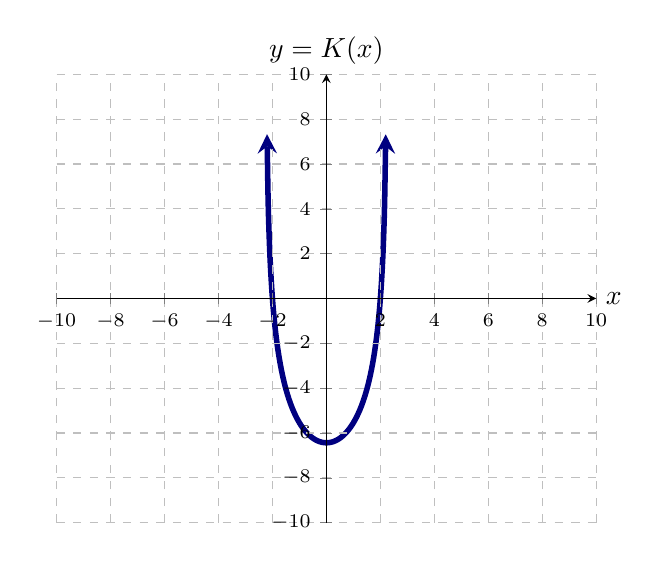
\begin{tikzpicture}
    \begin{axis}[name = sinax, domain=-10:10, ymax=10, xmax=10, ymin=-10, xmin=-10,
            axis lines =center, xlabel=$x$, ylabel={$y=K(x)$}, grid = major, grid style={dashed},
            ytick={-10,-8,-6,-4,-2,2,4,6,8,10},
            xtick={-10,-8,-6,-4,-2,2,4,6,8,10},
            yticklabels={$-10$,$-8$,$-6$,$-4$,$-2$,$2$,$4$,$6$,$8$,$10$}, 
            xticklabels={$-10$,$-8$,$-6$,$-4$,$-2$,$2$,$4$,$6$,$8$,$10$},
            ticklabel style={font=\scriptsize},
            every axis y label/.style={at=(current axis.above origin),anchor=south},
            every axis x label/.style={at=(current axis.right of origin),anchor=west},
            axis on top
          ]
          
          \addplot [line width=2, penColor, smooth,samples=100,domain=(-2.2:2.2),<->] ({x},{-4*ln(5 - x^2)});


           

    \end{axis}

\end{tikzpicture}
\end{image}























\begin{center}
\textbf{\textcolor{green!50!black}{ooooo-=-=-=-ooOoo-=-=-=-ooooo}} \\

more examples can be found by following this link\\ \link[More Examples of Composition]{https://ximera.osu.edu/csccmathematics/precalculus2/precalculus2/composition/examples/exampleList}

\end{center}





\end{document}
